\chapter{绪论}

\section{研究背景与意义}
% (Globe Union Centralab)
% (Texas Instruments,TI)
% (Integrated Circuit,IC)
% (Fairchild Semiconductor)
1947年,贝尔实验室发明了世界上第一个晶体管,时任全球联通公司中心实验室职员的杰克·基尔比(Jack Kilby)对此产生了浓厚兴趣,并于1958年在德州仪器创造了世界上第一个采用飞线连接的锗基底扩散工艺集成电路。紧接着,仙童半导体的罗伯特・诺伊斯(Robert Norton Noyce)在1959年发明了更具有实用价值的、能够进行大规模量产的、基于导线结构的硅基底平面工艺集成电路。此后,在短短的半个世纪内,集成电路无处不在。

作为第三次工业革命的起源,集成电路的发明和应用使人类社会从工业时代迈入了信息时代,极大的解放了生产力,推动了人类社会的发展。
早在集成电路发明早期,英特尔(Intel)的创始人之一戈登·摩尔(Gordon Earle Moore)就预言半导体行业将会迅猛发展,于1965年提出了著名的摩尔定律(Moore's law)\cite{moore_law_0}:集成电路上可容纳的晶体管数目,约每隔一年翻一番(1975年修正为两年\cite{moore_law_1})。不久后,罗伯特·登纳德(Robert Heath Dennard)发现,晶体管所消耗的电压和电流,会随着晶体管的尺寸做相同比例的减少,功率密度保持不变。这便是著名的登纳德缩放定律(Dennard scaling)\cite{dennard_scaling}。登纳德定律表明,由于单位面积的晶体管的功耗保持不变,而计算能力会随着每一代工艺节点而提升,芯片将会越来越节能。

\subsection{半导体工艺的发展}

近现代的数十年间,半导体制造商一直遵循着摩尔定律,不断缩小晶体管的尺寸,改进晶体管的制造方法\footnote{http://www.wecorp.com.cn/newsdetail.asp?newsid=152}。在传统的硅平面工艺被发明40年后,晶体管的栅极长度已经缩小到了100纳米(nanometer,nm)以下\cite{90nm_uniaxial_strained},由于短沟道效应(short-channel effects)的影响\cite{short-channel_effect}和工作电压的下降,载流子的界面散射加剧,迁移率降低,器件的驱动电流减小,响应速度变差。为了改善晶体管的开关特性,工业届各家厂商于2003年-2005年在90nm-65nm节点陆续引入了锗应变调控方法\cite{90nm_ge_strained,65nm_strained},实现了迁移率的大幅提升。之后,晶体管中电子的量子隧穿效应所引起的漏电流问题取代了性能问题,成为了首要考虑事项。为了降低发热,高介电常数金属栅极技术(High-k Metal Gate, HKMG)被Intel于2007年在45nm工艺节点采用\cite{45nm_hkmg},改进后被再次应用在32nm节点\cite{32nm_hkmg_2nd}。后来,为了进一步在减小晶体管尺寸的同时降低功耗,半导体制造厂商于2012年左右,在22nm及以下全面转向由加州大学伯克利分校的胡正明教授研发的鳍式场效应晶体管(Fin Field-Effect Transistor,FinFET)\cite{FinFET},延续着摩尔定律。然而,随着新工艺节点的不断推出,最新的量产工艺已经由台积电(Taiwan Semiconductor Manufacturing Company,TSMC)推进到了3nm,FinFET晶体管几乎达到了物理极限,摩尔定律陷入停滞。

\subsection{计算机体系结构的发展}

% (Clock frequency)
一方面,半导体制造厂商在不断地更新工艺制程以提高晶体管的密度;另一方面,芯片设计厂商也持续地从体系结构层面进行优化,以更好地利用额外增多的晶体管,改善芯片的性能、功耗和面积(Performance,Power,Area,即PPA)。在登纳德定律的指导下,早期的集成电路设计厂商孜孜不倦地提高芯片的时钟频率,实现性能更高的单核处理器。英特尔甚至在2000年豪言要在2011年将其生产的中央处理器(Central Processing Unit,CPU)推进至10GHz (Gigahertz)。然而,随着晶体管尺寸的持续缩小,电子的量子隧穿效应(Quantum tunneling effect)开始显露,晶体管的漏电流不断增加,功耗不减反增,登纳德定律开始失效,人们无法再简单的通过增加芯片的时钟频率来提高单核芯片的性能。同时,人们意识到,更高的时钟频率并不一定会带来芯片性能的增强。在1986年-2002年左右,伴随着主频提升的指令级并行(Instruction Level Parallelism,ILP)是提高处理器性能的主要方法。然而,过深的流水线会导致分支预测(Branch prediction)出错时,需要花费巨大的代价来恢复状态,平白消耗很多能量,带来不可忽视的性能损失\cite{new_golden}。
另外,虽然单核处理器性能每年以50\%的速度进行提升,但内存性能的提升每年仅约7\%,这导致了冯·诺依曼结构(Von Neumann architecture)\cite{von_arch}下严重的内存墙问题(The memory wall problem)\cite{memory_wall},考虑到内存访问所需要的时间远大于CPU的计算时间,盲目提升处理器主频作用非常有限。同时,随着互联网的快速发展,计算应用的类型从传统的计算密集型向数据密集型转变,这一方面使控制流变得不规则,导致难以有效利用ILP技术提升性能;另一方面导致了大量的数据移动,加剧了内存墙问题带来的负面影响\footnote{https://blog.51cto.com/echo1937/1294895}。
最后,芯片互连线延迟所占比例的持续上升和设计复杂度的不断增加也迫使研究人员停止开发更高速的单核处理器,转而将目光朝向多核架构的研究\cite{free_lauch_over}。2005年,以英特尔放弃研发4GHz的奔腾四(Pentium IV)处理器为标志,多核设计开始兴起\cite{计算机体系结构基础},如图\ref{50yrs_processor_trend}所示\cite{50yrs_processor_trend}。

\begin{figure}[htb]
    \centering
    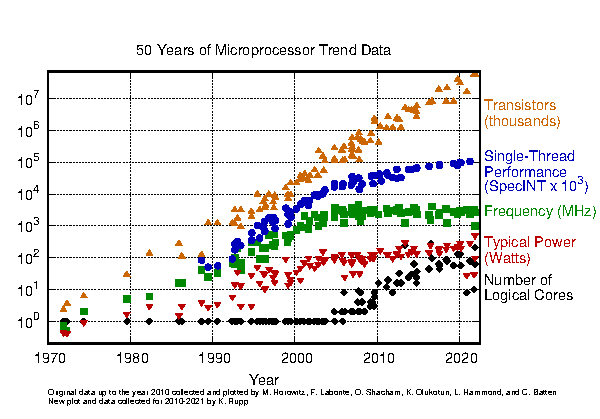
\includegraphics[width=\textwidth]{figs/50-years-processor-trend.pdf}
    \caption{近50年处理器发展趋势图}
    % \caption{近50年处理器发展趋势图\protect\footnotemark}
    \label{50yrs_processor_trend}
\end{figure}

多核架构的处理器拥有多个核心,能够同时运行多个任务,或者并行处理一个任务,大大缩短软件的运行时间。表面上看,不断增加芯片的核心数便能不断提高其处理能力。然而,多核处理器的运算能力并不能随着核数无限提升,主要有以下几个原因:(1) 由于功耗墙(The power wall)的存在,即使制造出一个拥有许多个核心的芯片,也无法允许所有核心同时运行\cite{dark_silicon},这部分不工作的晶体管被称为“暗硅(Dark silicon)”;(2)阿姆达尔定律表明\cite{amdahl_law},任务在多核处理器下的理论加速比的上限受限于任务中不能被并行处理的部分,公式定义如下:
\begin{equation}
    \label{amdahl_law}
    \text{加速比} = \frac{W_s+W_p}{W_s+ \frac{W_p}{p}}
\end{equation}
式中$W_s$和$W_p$为任务规模中的串行分量(不能被并行的部分)和并行分量(可以被并行的部分)。若程序没有并行分量,那么不论使用多少核的处理器,任务都无法被加速;(3)由于内存提升的速度赶不上处理器提升的速度且差距越来越大,导致了内存墙问题愈发严重。对某些应用来讲,盲目堆砌多核,不但不能加速任务的处理,反而导致性能的下降\cite{multicore_bad}。

% \footnotetext{https://github.com/karlrupp/microprocessor-trend-data}

为了解决多核架构遇到的问题,软件和硬件人员分别从两方面入手进行优化。一方面,与多核处理器配套的软件如操作系统和编译器等工具开始充分发展,尽可能利用多核架构的优点,提高任务的运行速度;另一方面,计算机体系结构人员开始采用不同的方法来解决“暗硅”问题和内存墙问题。对于内存墙问题,研究人员使用多级缓存(Multi-level caches)结构和更先进的分支预测方法来增加cache的命中率;对于“暗硅”问题,学术界和工业界提出了3个办法来充分利用未工作的晶体管\cite{is_dark_silicon}:(1)低速多核。把处理器的每个核的运行频率限制在一个较低的水平,充分利用处理器的并行性,提高运算能力,典型的例子包括英特尔的由太阳能供电的x86多核处理器\cite{solar_x86};(2)自动超频。允许多个核心在短时间内达到很高的频率用来处理高计算量的任务,之后迅速将每个核心的频率降低来减缓发热,常用于由电池供电的对功耗有严格要求的芯片;(3)专用加速器。把“暗硅”部分设计成专用处理器(Application-specific integrated circuit, ASIC),由于ASIC的性能高,发热低,可以和CPU结合提高处理能力。
为了设计能效更高的处理器,处理器厂商往往结合多种方法来进行优化,比如英特尔的睿频技术(Turbo Boost Technology)\cite{intel_turbo_boost},ARM的大小核架构(big.LITTLE)\cite{arm_big_little}等。发展到现代,广义上的处理器已经不仅仅是一个只有传统运算核心的芯片,而是成为了一个包含许多专用处理单元如GPU(Graphics Processing Unit)、NPU(Neural Processing Units)、ISP(Image Signal Processor)、嵌入式FPGA(embedded Field Programmable Gate Array,eFPGA)、DSP(Digital Signal Processing)等模块的复杂异构片上系统(System on Chip,SoC)。

随着机器学习(Machine Learning,ML)的飞速发展,人工智能(Artificial Intelligence, AI)模型对算力的需求激增。在2012年之前,训练一个ML系统所需的算力大约每17到29个月翻一番\cite{AI:computing_demand_trend},增长率和摩尔定律基本一致。然而,2012年杰弗里·辛顿(Geoffrey Everest Hinton)的学生亚历克斯·克里泽夫斯基(Alex Krizhevsky)设计了AlexNet\cite{AI:AlexNet}这一8层卷积神经网络(Convolutional Neural Network,CNN),利用GPU夺得的ImageNet LSVRC(Large Scale Visual Recognition Challenge)竞赛的冠军,并大幅领先第二名10.8个百分点,掀起了CNN研究的热潮,深度学习(Deep Learning)迎来了大爆发。伴随着互联网的快速发展和全球社会的数字化转型带来的海量数据,深度学习常规模型(Regular-scale Model)训练一次所需的算力大约每4-9个月翻一番\cite{AI:computing_demand_trend}。同时,随着2016年以谷歌(Google)的AlphaGo\cite{AI:AlphaGo}4:1战胜了韩国棋手李世石为代表,大规模模型(Large-Scale Model)开始引领人工智能的潮流,计算量大约每9到10个月翻一番\cite{AI:computing_demand_trend}。如此巨大的算力需求是传统的CPU和GPU处理器所无能为力的,于是各种领域专用架构(Domain-Specific Architecture,DSA)竞相涌现,牺牲了部分通用性,实现高能效计算,如寒武纪的DianNao\cite{Accelerator:DianNao}、Google的已经发展到第四代的TPU(Tensor Processing Unit)\cite{Accelerator:TPU}、GraphCore的IPU(Intelligence Processing Unit)\cite{Accelerator:IPU}、华为的DaVinci架构\cite{Accelerator:DaVinci}、百度的昆仑芯片\cite{Accelerator:Kunlun}等,计算机架构迎来了新黄金时代\cite{new_golden}。与ASIC相比,DSA的通用性更强,以适应日新月异的AI算法。
同时,CPU、GPU和FPGA架构也不断革新,引入了各种针对ML应用的专用处理单元,如Intel至强(Xeon)处理器中的AI加速单元\cite{Accelerator:intel_xeon_4th}、英伟达(Nvidia)GPU中的张量计算核心(Tensor Core)\cite{Accelerator:nvdia_h100_tensor_core_4th}、AMD的FPGA中的AI引擎(AI Engine,AIE)\cite{Accelerator:amd_versal_AIE}。

与计算机视觉(Computer Vision,CV)领域不同,在自然语言处理(Natural Language Processing,NLP)方面,纯粹由注意力机制构成的Transformer模型\cite{AI:attention_is_all}取代了CNN,占据了主导地位。在Transformer被Google提出的一年后,大规模语言模型(Large Language Model,LLM)开始出现。以OpenAI旗下的GPT(Generative Pre-trained Transformer)为代表,LLM的大小一直在飞速增长。2018年发布的GPT-1参数量为1.17亿,数据量为5GB(Gigabyte);2019年的GPT-2参数量为15亿,数据量为40GB;2020年的GPT-3参数量为1750亿,数据量增加到45TB(Terabyte)。研究表明,Transformer类模型训练所需的运算量每2年增加750倍\cite{ai_and_memory_wall},远超摩尔定律的演进速率,如图\ref{AI:ai_and_compute}所示。

\begin{figure}[htb]
    \centering
    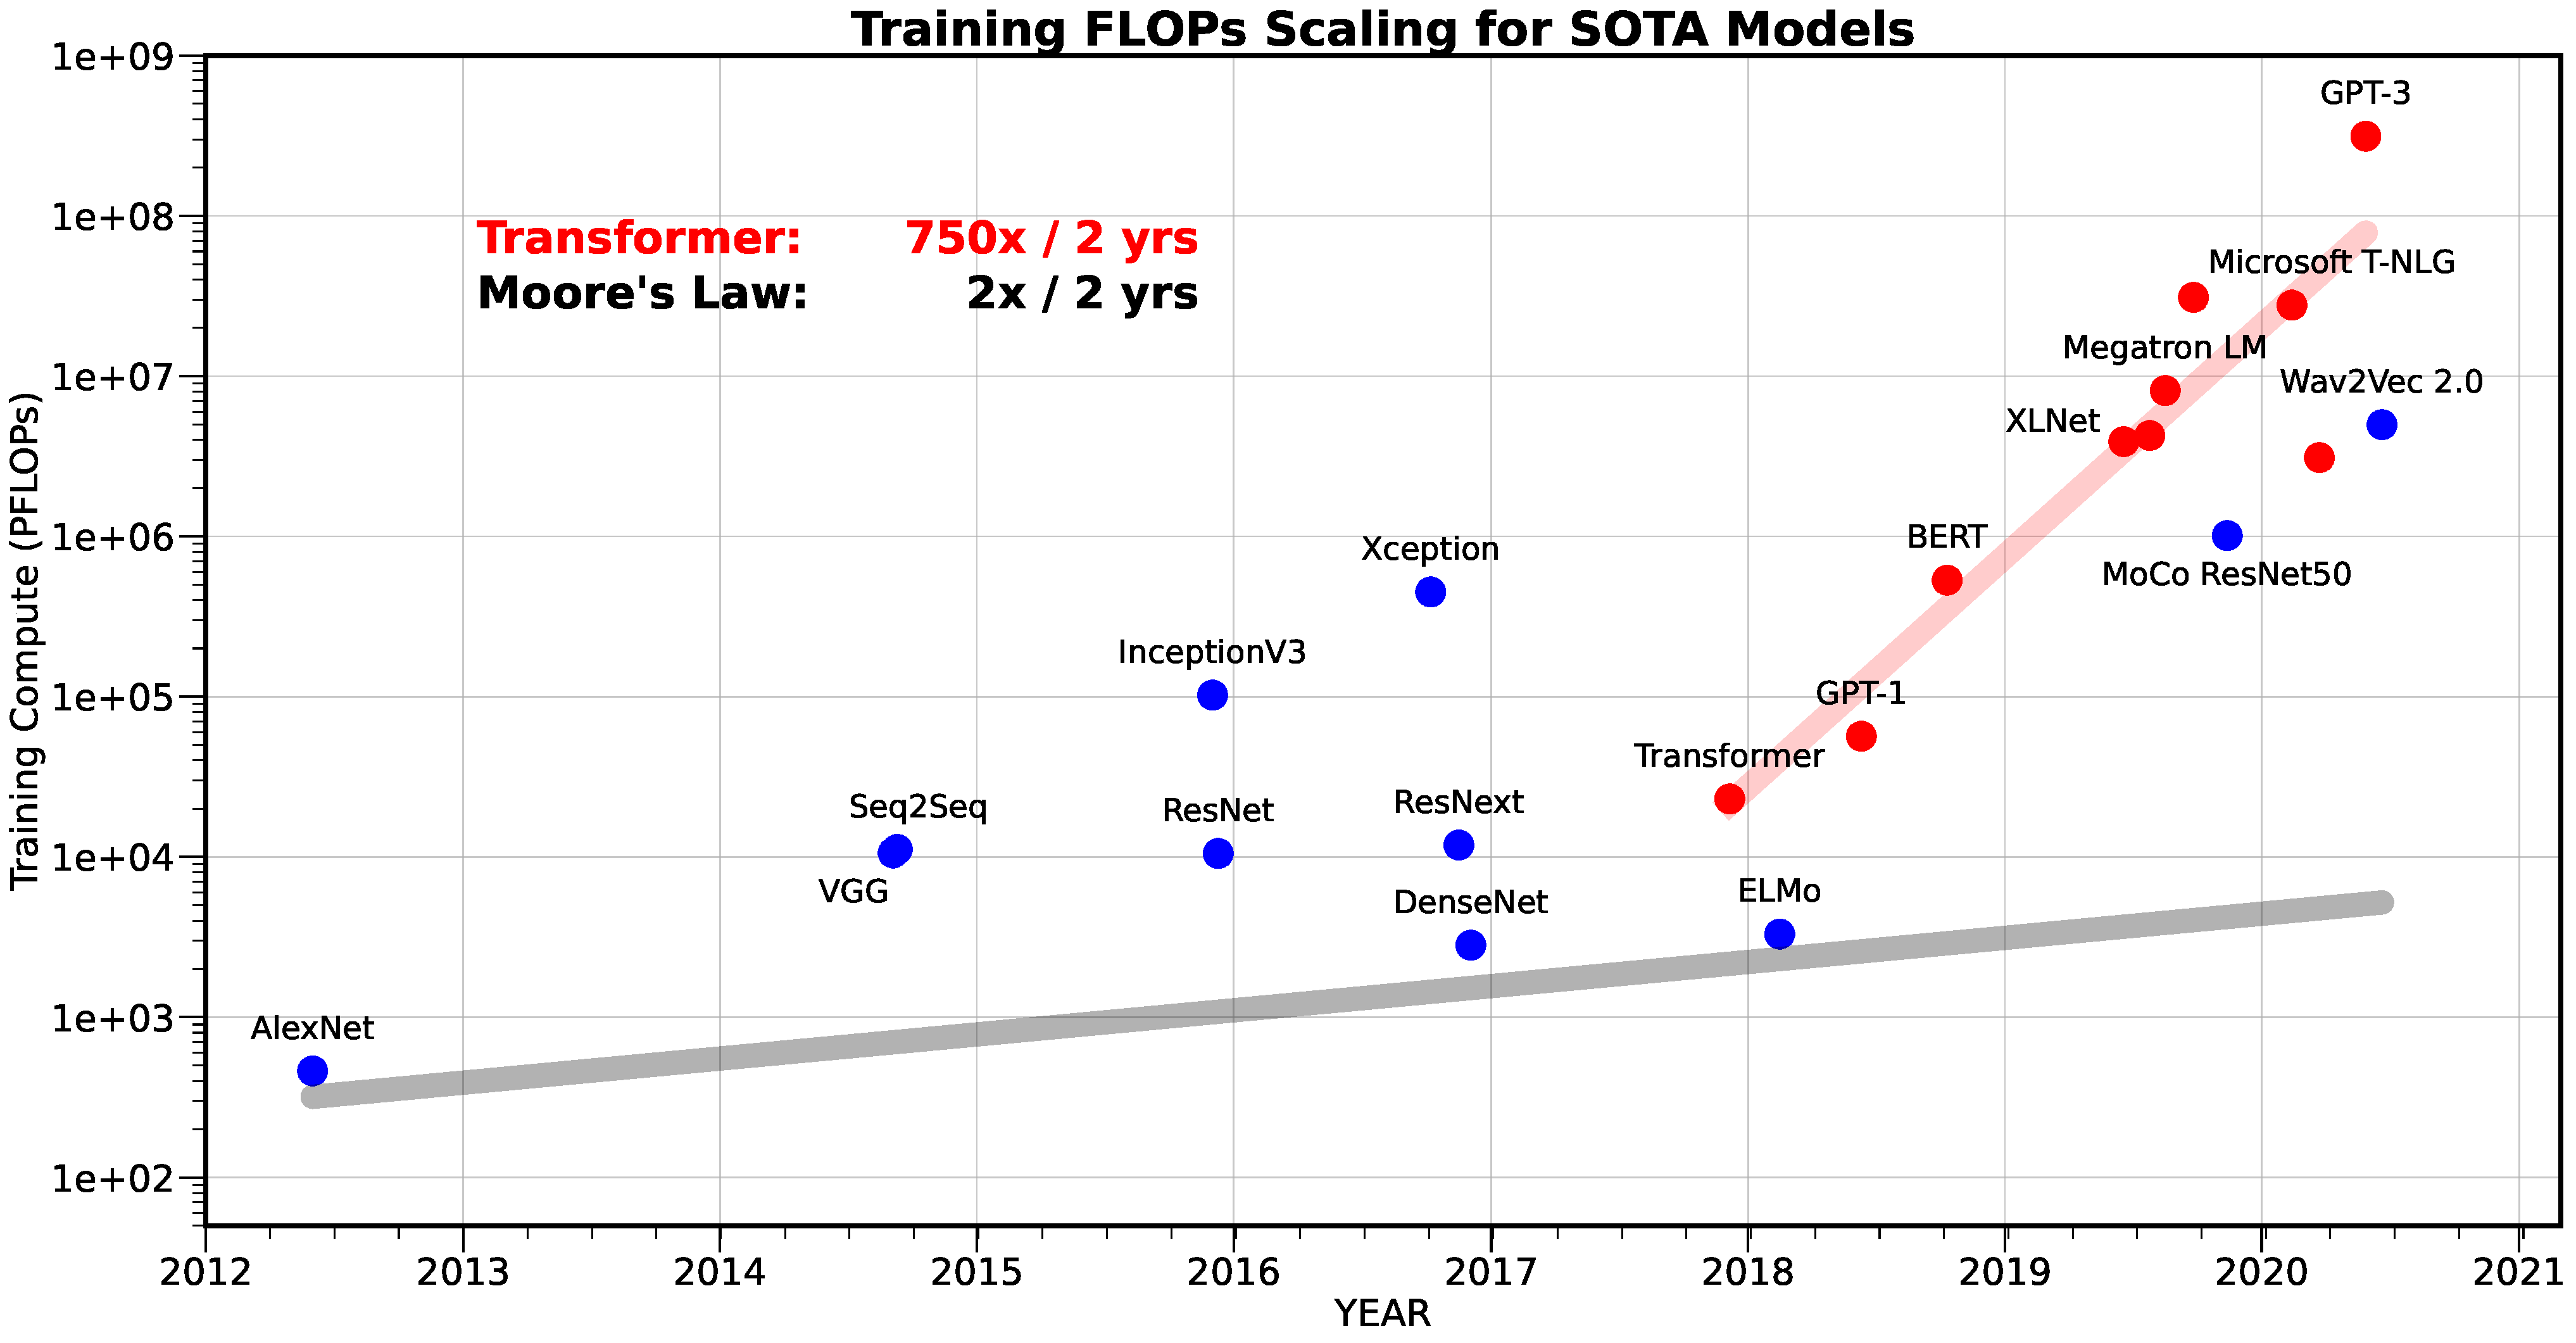
\includegraphics[width=\textwidth]{figs/AI-Fig-ai_and_compute.pdf}
    \caption{Transformer类模型训练所需的运算量}
    \label{AI:ai_and_compute}
\end{figure}


如此巨大的计算需求,需要海量的算力进行支撑。目前业界通用的办法是利用并行化技术在多个GPU或DSA上进行训练,以求在合理的时间内获得想要的结果。然而,这会伴随着资源的大量消耗。例如,训练一个GPT-3模型需要355个GPU年(一块GPU运行355年的运算量),花费460万美元,耗电1287兆瓦时(Megawatt Hour,MWh),大约相当于120个家庭1年的用电量\cite{AI:carbon_google_2021,AI:zeus},并且,训练阶段的能耗通常只占模型整个生命周期的40\%\cite{AI:carbon_google_2022},ChatGPT的火热导致这一占比对GPT类应用更低。这产生了大量碳排放,对环境造成了很大的负担。为了降低能耗,研究人员从算法和硬件两方面来对AI应用进行优化。一方面,高效的ML模型架构可以在更少计算量的情况下实现更高的精度,减少资源的消耗;另一方面,采用专门用于AI训练和推断的处理器可以提高系统的能效,实现绿色计算(Green Computing)\cite{AI:green_computing}。但是,目前的研究表明,LLM模型的规模越大,往往NLP任务的效果越好,\cite{AI:llm_overview},这意味着模型的精简程度十分有限。同时,芯片的能效提升远远跟不上模型的规模增长,人们仍然希望能有新的方法在提升算力的同时降低能源消耗。


\subsection{后摩尔时代的技术路线}

以生成式AI(Generative AI)为代表的人工智能等应用的发展,对半导体材料和器件提出了更高的性能要求。当前,随着硅晶体管的尺寸接近物理极限,不仅特征尺寸的缩小越来越困难,迭代产生的工艺红利也消失殆尽,硅基电子技术临近生命周期极限。为了探索集成电路领域新的发展规律,持续提高芯片能效,学术界和工业界提出了多个发展方向,这里列举几个典型的技术路线:

% \footnote{https://irds.ieee.org/editions/2022}

(1)More Moore

“More Moore”即“深度摩尔”,基本思路是延续摩尔定律的发展,在兼顾性能和功耗的同时,继续缩小晶体管的尺寸\cite{more_moore}。随着FinFET的漏电越发严重,对沟道拥有更强控制能力的全环栅晶体管(Gate All Around FET,GAAFET)将成为未来主流的晶体管结构\cite{GAA}。

(2)More than Moore

“More than Moore”即“超越摩尔”,是指依靠电路设计以及系统协同优化,通过先进封装技术以提升芯片性能\cite{more_than_moore}。与不断优化晶体管的“More Moore”路线不同,“More than Moore”从需求端出发,以系统应用为起点,尝试在提高芯片的集成度的同时降低芯片制造的成本。在SoC中,除了逻辑(Logic)和存储(Dynamic Random Access Memory,DRAM)部分以外,模拟(Analog)、射频(Radio Frequency,RF)等模块往往并不能随着工艺的迭代获得显著地性能改善。因此,数字(Digital)部分可由先进工艺实现,而其余部分可选择更合适的工艺进行流片,最后不同模块通过先进封装技术组合在一起,模块间通过高速接口进行通讯。


(3)Beyond Complementary Metal Oxide Semiconductor(CMOS)

前面两种路线仍然是基于硅基集成电路进行拓展,“Beyond CMOS”是指利用CMOS之外的新器件、新材料来制造晶体管,提升芯片的性能\cite{beyond_cmos}。与CMOS相比,这类新器件往往具有更高的密度、更强的性能、更低的功耗,但可能还无法大规模制造或制造成本不可接受。目前,该方向是学术界和工业界研究的热点之一,各种各样的新型方案百花齐放,比如具有低功耗的隧穿场效应晶体管(Tunneling FET,TFET)\cite{TFET}、与CMOS工艺兼容的单电子晶体管(Single Electron Transistor,SET)\cite{SET}、具有高迁移率的石墨烯晶体管(Graphene Transistor)\cite{Graphene_transistor}、适合RF电路的碳纳米管场效应晶体管(Carbon Nanotube FET,CNFET)\cite{Carbon_Nanotube_FET}等。但是,这一方向的绝大多数成果还未走出实验室,仍处于初期的前瞻性研究阶段,距离商业化较远。

\subsection{近似计算的优势} \label{approximate_computing_advance}

不论是可穿戴设备、便携设备还是数据中心,集成电路面临的功耗问题日益严峻,人们需要寻找新的芯片设计方法以同时满足高性能和低功耗的严苛要求。
在实际生活中,许多应用具有错误容忍的特性,这类应用被称为容错应用(Error-tolerant applications)。一个典型的例子是,当观看视频时,由于人类感知的限制,即使视频中某些帧出错甚至丢失了,人类很可能也察觉不到。类似地,即使搜索引擎返回的结果没那么精确,查询者也可以接受。
近似计算(Approximate computing)是一种新型的计算范式(Paradigm),与精确计算(Exact computing)相比,它可能返回不准确的结果。与容错应用结合,近似计算可以在满足精度需求的前提下节省大量能源,达到降低功耗、提高能效的目的。
因此,在数字信号处理、机器学习等场景中,近似计算得到了工业界和学术界的广泛关注\cite{AC:survey:survey's_survey,AC:survey:hanjie_2013_ETS}。

目前,有关近似计算的研究主要集中在四个层面:

(1)软件层近似(Software-level approximation)

软件层的近似有多种实现方式,比如在循环中跳过一些迭代来更快地获得计算结果,或者根据条件语句进行判断,从而跳过某些任务的执行来减少程序运行时间。另外,许多启发式算法(Heuristic algorithm)如模拟退火(Simulated annealing)和遗传算法(Genetic algorithm)常常需要在一定的时间内获得次优解(Sub-optimal solution),这也是软件层近似的一种。

(2)近似电路(Approximate circuits):

通过对加法器(Adder)\cite{AC:Aadd:simple_yet}、乘法器(Multiplier)\cite{AC:AM:Adapt}、除法器(Divider)\cite{AC:Div:2019dac}等算术运算单元(Arithmetic units)引入近似,获得能效的提升,被称为电路级近似。电路级近似的实现方式大体上可以分为两类:电压调节(Voltage scaling)和功能近似(Functional approximation)\cite{AC:ALS:survey}。其中,电压调节是通过降低模块的工作电压但不降低频率来减少电路的功耗。然而,这一般会产生时序错误(Timing error),带来难以控制的计算误差\cite{AC:Arith:overscale}。功能近似通常聚焦在电路结构或门级网表(Gate-level netlist)的简化上,与电压调节相比,功能近似的方法带来的误差易于控制,也是目前近似计算研究最为深入的方向\cite{AC:Arith:survey_hanjie}。

(3)近似存储和近似内存(Approximate storage and memory):

与存储精确数据相比,近似存储能够改善数据读取的延迟,降低数据搬移的能耗。例如,通过舍弃浮点数(Floating-point number)低有效位(the Least Significant Bit,LSB),可以减少数据存储所需要的位宽(Bit width),提高存储密度。在基于Flash的固态硬盘(Solid State Drive,SSD)中引入近似计算可以提高SSD的读取性能\cite{AC:Store:ASCache}。对于内存或cache来说,降低DRAM的刷新率\cite{AC:Store:DRAM}或静态随机存储器(Static Random-Access Memory,SRAM)\cite{AC:Store:SRAM}的供电电压也可以达到节省功耗的目的。

(4)近似系统(Approximate system):

在近似系统中,对不同子模块包括传感器、内存、处理器、通信接口等协同优化,可以取得比单独优化各个组件更好的效果\cite{AC:Sys:camera}。


% \section{国内外研究现状}


\section{本文主要工作及组织结构}

本文的工作主要集中在近似电路中定点数(Fixed-point number)乘法器的设计及应用上,包括以下三个方面的研究:(1)基于白盒优化的考虑输入分布(Input distribution)和极性(Polarity)的面向ASIC的自动化近似乘法器设计方法;(2)基于黑盒优化的面向FPGA的自动化近似乘法器设计方法;(3)基于生成的近似乘法器库进行近似逻辑综合(Approximate Logic Synthesis,ALS)\cite{AC:ALS:survey}的研究。具体工作如下:

(1)面向ASIC,提出并开源了一个白盒优化的考虑输入分布和极性的高质量近似乘法器自动化生成方法,该方法通过减少乘法器部分积(Partial product)的规模来实现PPA的提升。在对部分积进行累加求和之前,引入与(AND)、或(OR)、异或(XOR)和移位(Shift)操作,降低部分积的个数。具体来说,基于应用驱动,统计应用中乘法器的输入数据分布,并在考虑极性的情况下进行部分积的压缩,以减轻后续累加的负担。为了能够自动化求解,将寻找较优压缩操作的问题建模成数学问题,并用 MATLAB 对其进行求解。
另外,基于改进的Baugh-Wooley算法\cite{EM:baugh-wooley,EM:baugh-wooley_modified_PP_reorga,EM:baugh-wooley_diff},方法经过扩展后实现了对补码有符号乘法器的支持。基于位宽为$8\times8$无符号乘法的三个不同规模的神经网络包括LeNet、AlexNet和VGG16以及位宽为$16\times16$有符号定点数乘法的有限冲击响应(Finite Impulse Response,FIR)滤波器的实验结果表明,与国际前沿工作相比,生成的近似乘法器在几乎没有精度损失的前提下,实现26.4\%-27.1\%的功耗延迟面积积(Product of Power,Delay,and Area,PDA)提升。

(2)面向FPGA,设计并开源了一个基于黑盒优化的近似乘法器生成器,该方法通过优化乘法器部分积的累加电路实现。首先,假设累加电路的第一步是用半加器(Half adder)进行初始求和,自动化生成任意位宽精确乘法器的半加器电路,计算每个半加器的权重,同时保留后续的粗粒度加法;之后,利用开源Verilog解析工具Yosys\cite{LS:yosys}将半加器阵列映射成门级网表,保留每个半加器的权重;同时,对每个半加器设计搜索空间,分为删减(Eliminate)、或之和(OR $Sum$)、直接进位(Direct $Cout$)、精确(Exact)四种;紧接着,为了将多目标优化问题建模为单目标优化问题,详细设计目标函数($cost$ function)以综合考虑硬件PPA和软件精度;最后,基于给定的面积改善比例和半加器的权重,利用并行贝叶斯优化(Bayesian optimization)算法对生成的空间进行探索,生成高质量的乘法器集合。与国际前沿工作中1167个近似乘法器相比,生成的乘法器综合指标平均提升28.70\%-38.47\%,且处于帕累托前沿(Pareto front)。

(3)基于前面两种自动化方法得到的ASIC和FPGA乘法器库,首先针对传统逻辑综合,提出并开源了一个基于MFFC(Maximum Fanout-Free Cone)自适应超图划分的强化学习(Reinforcement learning)逻辑优化序列探索框架,与ABC\cite{LS:ABC}的resyn2相比,超过150个电路的DC(Design Compiler)结果表明,面积延迟积(Area Delay Product,ADP)平均提高了5.17\%;接着将序列探索与近似逻辑综合\cite{AC:ALS:survey}结合,基于给定的近似单元库,在对电路中的乘法器模块进行替代之后通过探索框架进行优化,探究不同近似乘法器对DNN加速器的硬件实现带来的影响,实现整体PPA的提升。

本文共有六个章节,各章节的组织结构安排如下:

第一章,绪论。首先介绍了自集成电路发明以来半导体工艺和计算机体系结构的发展,之后分析了近似计算对容错应用具有的优势,引出本文的研究目的,同时简述了本文的主要工作和创新点。

第二章,乘法器概述。首先介绍了精确定点数乘法器的运算过程及不同的实现方法,以及采用Mitchell近似的对数乘法器\cite{EM:mitchell};之后阐述了目前主流的衡量近似电路(主要是算术单元)误差的指标,这些指标同样适用于近似乘法器。

第三章,ASIC近似乘法器设计。首先分析了国内外有关ASIC近似乘法器的实现方法,主要分为四大类:手工设计(Manual design)、数学转换近似(Mathematical transformation approximation)、自动化方法(Automated method)、近似电路综合(Approximate circuit synthesis);接着介绍了基于白盒优化的考虑数据分布和输入极性的自动化近似乘法器设计方法,并与国际前沿工作进行对比。

第四章,FPGA近似乘法器设计。首先介绍了学术界提出的面向FPGA领域的多种近似乘法器设计方法,主要是通过手工修改查找表(LookUp Table,LUT)编码的方式实现;接着提出了基于黑盒优化的自动化近似乘法器生成器,并与国际前沿工作进行硬件PPA和软件精度比较。

第五章,近似逻辑综合。首先介绍了传统的逻辑综合,设计并实现了一个基于MFFC(Maximum Fanout-Free Cone)自适应超图划分的强化学习逻辑优化序列探索框架,并与已有的逻辑综合探索框架进行对比;之后与近似逻辑综合结合,基于提出的近似乘法器库针对DNN加速器将电路中的乘法器模块与非乘法器部分协同优化,探究不同乘法器对加速器硬件实现带来的影响,提高电路的PPA。

第六章,总结与展望。该章节总结了本文的主要研究工作和成果,分析了工作中存在的局限性,并对未来进一步的探索方向进行了展望。

